\documentclass{report}
\usepackage[margin=1in, paperwidth=8.5in, paperheight=11in]{geometry}
%Math packages%
\usepackage{amsmath}
\usepackage{amsthm}
%Spacing%
\usepackage{setspace}
%Package to adjust indentation%
\usepackage{changepage}
\onehalfspacing
%Lecture number%
\newcommand{\lectureNum}{19}
%Variables - Date and Course%
\newcommand{\curDate}{March 16, 2017}
\newcommand{\course}{CS 240}
%Defining the example tag%
%\theoremstyle{definition}%
\newtheorem{ex}{Example}[section]
%Setting counter given the lecture number%
\setcounter{chapter}{\lectureNum{}}
%Package to insert code%
\usepackage{listings}
\usepackage{courier}
\usepackage{xcolor}
\lstset { 
    tabsize=2,
    breaklines=true,
    language=C++,
    backgroundcolor=\color{blue!8}, % set backgroundcolor
    basicstyle=\footnotesize\ttfamily,% basic font setting
}
%Package to draw trees%
\usepackage{tikz}


\begin{document}
%Note title%
\begin{center}
\begin{Large}
\textsc{\course{} | Lecture \lectureNum{}}
\end{Large}
\end{center} 
\noindent \textit{Bartosz Antczak} \hfill
\textit{Instructor: Eric Schost} \hfill
\textit{\curDate{}}
\rule{\textwidth}{0.4pt}
% Actual Notes%
\section{Rabin-Karp Fingerprint Algorithm}
The main idea behind this algorithm is to use hashing. We compute the hash function for each text position.
\subsection{Overview}
We define a fixed value $n$ for our hash ``table". We then define our search pattern and our search text. With that, we define our hash function $h(x) = x \mod n$. We will use this hash function on every substring of the same size as our pattern. Once we arrive at a substring whose hash function matches the hash function of the pattern, we verify that the strings match: if they do, we found it; otherwise, we keep searching.
\subsection{A Problem Occurs}
Note that the runtime of the defined algorithm is $\Theta(mn)$, which is no better than brute force.
\subsection{The Solution Arrives}
Two brave men, Rabin and Karp, discovered a way to update the hashes of every substring in constant time! \textit{(P = NP confirmed)}.
The idea is use the hash from the previous substring to compute the next one! The runtime is $O(1)$ per hash, except the first one.
The way we compute it is as follows:
\begin{figure}[ht]
\begin{center}
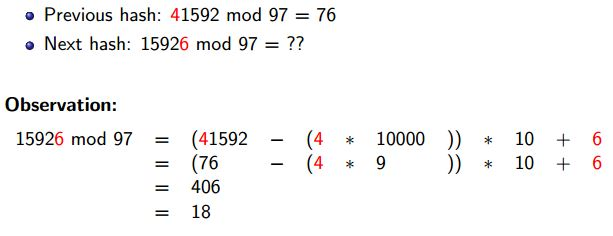
\includegraphics[scale=0.7]{comp.jpg}7
\end{center}
\end{figure}
It is recommended to choose a random large prime number as your hash table size.
\section{Suffix Tries and Suffix Trees}
What if we want to search for many patterns $P$ within the same fixed text $T$? Here, we can preprocess the text $T$ rather the the pattern $P$. From this, we make an observation:
\begin{center}
\textit{P is a substring of T $\iff$ P is a prefix of some suffix of T}
\end{center}
\subsection{Definition | Suffix Trie and Suffix Tree}
A \textbf{suffix trie} is a trie that stores all suffixes of a text $T$. A \textbf{suffix tree} is the compressed suffix trie of $T$.

%END%
\end{document}